%------------------------------------------------
%
% RequestFulfillment.tex 
%
% This section introduces the request fulfillment
% process.
%------------------------------------------------
\section[Request Fulfillment]{request fulfillment}
\label{prc-request}
Il termine \english{Service Request} è utilizzato come generica descrizione per differenti richieste provenienti dagli utenti verso la funzione di \english{Service Desk}.

Molte di queste richieste riguardano piccoli cambiamenti, a basso impatto, che si verificano di frequente. Esempi di queste richieste di servizi includono:

\begin{itemize}
\item{l'installazione di \english{software} aggiuntivo su una particolare \english{workstation};}
\item{la richiesta di spostare alcuni oggetti dal \english{desktop} dell'utente;}
\item{la richiesta di informazioni.}
\end{itemize}

Data la loro dimensione, frequenza ed il basso impatto che possiedono significa il posto più corretto dove gestirle è in un processo separato invece di congestionare i processi di \ac{Incident-Management} e \ac{Change-Management}. Questo processo prende il nome di \acf{Request-Fulfillment}.

\subsection[Scopo e portata del processo]{scopo e portata del processo}
\label{prc-request-scope}
Il processo di \ac{Request-Fulfillment} è il processo dove vengono gestite le richieste di servizio da parte degli utenti. Gli obiettivi includono:

\begin{itemize}
\item{fornire agli utenti un canale presso cui possano richiedere e successivamente ricevere servizi standard per i quali esiste un processo di approvazione e qualificazione predefinito;}
\item{fornire agli utenti/clienti informazioni sulla disponibilità dei servizi e come ottenerli;}
\item{per reperire e fornire i componenti di servizi standard (quali ad esempio licenze);}
\item{per assistere con informazioni generali, complementi o commenti gli utenti/clienti.}
\end{itemize}

Le attività necessarie al soddisfacimento di una richiesta variano a seconda di ciò che viene richiesto ma generalmente può essere suddiviso in una serie di attività che devono essere eseguite.

Le richieste devono essere gestiti in modo diverso dagli incidenti, questi ultimi sono imprevisti mentre le richieste di servizio sono un'entità che può e deve essere pianificata.

Molte richieste di servizio possono e devono essere gestite dal \english{Service Desk} fintanto che hanno risorse sufficienti, il tempo, gli strumenti e le competenze.

\subsection[Valore del processo]{valore del processo}
\label{prc-request-value}
Il \english{business} riceve valore da questo processo se esso fornisce risposte veloci ed effettivo accesso ai servizi necessari agli utenti per migliorare la loro produttività.

Ha lo scopo di ridurre la burocrazia necessaria per richiedere e ricevere accesso a servizi nuovi o già esistenti riducendo cosi il costo di fornitura.

La centralizzazione di questo processo consente inoltre di aumentare il livello di controllo su di essi.

\subsection[attività]{attività}
\label{prc-request-activities}
Le richieste di servizio possono essere richieste attraverso la funzione di \english{Service Desk}, tuttavia il processo offre l'opportunità agli utenti di selezionare, in una apposita interfaccia web, quale servizio essi richiedano gli venga concesso. Questa attività prende il nome di \keyword{selezione da menù}.

Se nell'interfaccia web non dovesse essere presente il servizio che gli utenti richiedono essi possono compilare un \english{form} in cui esplicitano le loro necessità.

\begin{figure}[htbp]
\centering
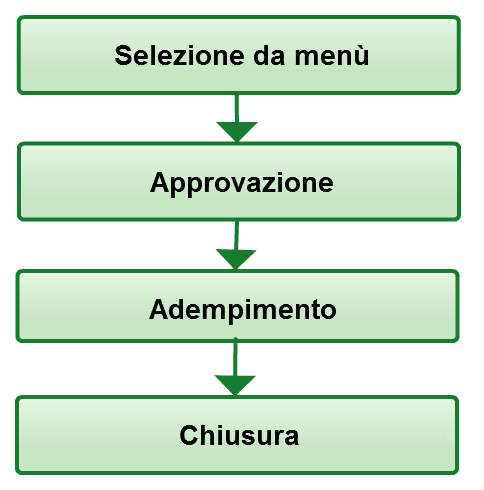
\includegraphics[scale=0.5]{Images/Diagrams/Request_fulfillment.png}
\caption{Attività del processo di \english{Request Fulfillment}}
\label{prc-request-activities-img}
\end{figure}

Le richieste che giungono al \english{Service Desk} sono di due tipologie:

\begin{itemize}
\item{approvate;}
\item{soggette ad approvazione;}
\end{itemize}

Quelle approvate possono essere automaticamente erogate agli utenti mentre quelle soggette ad approvazione hanno bisogno di ulteriori passi per ottenere l'approvazione finanziaria. In quest'ultimo caso il compito dello staff del \english{Service Desk} dovrà mantenere aggiornato l'utente sullo stato della richiesta, in particolare dovrà comunicare ad esso se la richiesta viene o meno approvata.

Durante l'attività di \keyword{adempimento} il responsabile della richiesta, presso il \english{Service Desk}, ha il compito di implementare e rendere disponibile all'utente il servizio di cui ha bisogno.

Al termine dell'implementazione il responsabile ha il compito di tracciare ogni attività presso la banca dati del \english{Service Desk} e marcare la richiesta come \keyword{chiusa}.